\documentclass[12pt]{article}
\usepackage[utf8]{inputenc}
\usepackage{float}
\usepackage{amsmath}
\usepackage{tikz}

\usepackage[hmargin=3cm,vmargin=6.0cm]{geometry}
%\topmargin=0cm
\topmargin=-2cm
\addtolength{\textheight}{6.5cm}
\addtolength{\textwidth}{2.0cm}
%\setlength{\leftmargin}{-5cm}
\setlength{\oddsidemargin}{0.0cm}
\setlength{\evensidemargin}{0.0cm}

\begin{document}

\section*{Student Information } 

Full Name : Mehmet Rüçhan Yavuzdemir \\
Id Number : 2522159 \\

\section*{Answer 1}

Let f(x) be  $\sum_{n=0}^{\infty} a_n x^n$.\\\\

$a_n = 3a_{n-1} + 4a_{n-2}$, n $\geq$ 2\\\\

$\sum_{n=2}^{\infty} a_n x^n$ = 3 $\sum_{n=2}^{\infty} a_{n-1}x^n$ + 4$\sum_{n=2}^{\infty} a_{n-2} x^n$\\\\

$\sum_{n=0}^{\infty} a_n x^n - a_0 - a_1x$  = $3x \sum_{n=2}^{\infty} a_{n-1}x^{n-1}$ + $4x^2\sum_{n=2}^{\infty} a_{n-2} x^{n-2}$\\\\

$\sum_{n=0}^{\infty} a_n x^n - a_0 - a_1x$  = $3x \sum_{n=1}^{\infty} a_{n}x^{n}$ + $4x^2\sum_{n=0}^{\infty} a_{n} x^{n}$\\\\

$\sum_{n=0}^{\infty} a_n x^n- a_0 - a_1x = 3x(\sum_{n=0}^{\infty} a_n x^n-a_0) + 4x^2\sum_{n=0}^{\infty} a_n x^n$\\\\

$f(x)- a_0 - a_1x = 3x(f(x)-a_0) + 4x^2f(x)$\\\\

$a_0 = 1$, $a_1 = 1$\\\\

$f(x) -x -1= 3x(f(x)-1) + 4x^2(f(x))$\\\\

$(4x^2 +3x -1)f(x) = 2x-1$\\\\

$f(x) = \frac{2x-1}{4x^2 +3x -1} = \frac{2x-1}{(4x-1)(x+1)}$\\\\

$= \frac{2x-1}{(4x-1)(x+1)} = \frac{A}{4x-1} + \frac{B}{x+1}$\\\\

$2x-1 = Ax + A + 4Bx - B$\\\\
$A-B = -1$\\
$A+4B = 2$\\
$A = -0.4$\\
$B = 0.6$\\

$f(x) = 0.4 \frac{1}{1-4x} + 0.6 \frac{1}{1+x}$\\\\

$\sum_{n=0}^{\infty}x^n = \frac{1}{1-x}$ for $|x| \leq 1$\\\\
$x \leftarrow 4x$\\
$\sum_{n=0}^{\infty}(4x)^n = \frac{1}{1-4x}$ for $|x| \leq 0.25$\\\\
$x \leftarrow -x$\\
$\sum_{n=0}^{\infty}(-x)^n = \frac{1}{1-(-x)} = \frac{1}{1+x}$ for $|x| \leq 1$\\\\

$f(x) = 0.4\sum_{n=0}^{\infty}(4x)^n + 0.6\sum_{n=0}^{\infty}(-x)^n$\\\\

$f(x) = 0.4\sum_{n=0}^{\infty}4^n x^n + 0.6\sum_{n=0}^{\infty} (-1)^n x^n$\\\\

Remember that $f(x)$ was $\sum_{n=0}^{\infty} a_n x^n$. Hence, $a_n = 0.4 (4)^n + 0.6 (-1)^n$.

Generating function: $$<1,1,7,25,103,...>$$

\section*{Answer 2}
\subsection*{a) }
Let s = $<2,5,11,29,83,245>$, it can be written as the sum of two sequences.
It seems that we have an additional 2 except for the first term. We are going to subtract 2 from each term and apply a right shift to get the sequence in a general form.\\\\

Remember that $<1,1,1,1,1,1...>$ is nothing but $\sum_{n=0}^{\infty}x^n$.\\\\

$\sum_{n=0}^{\infty}x^n = \frac{1}{1-x}$ for $|x| \leq 1$\\\\

If we multiply each term by two, $<2,2,2,2,2,2...>$ = $\frac{2}{1-x}$\\\\

$s$ = $<2,2,2,2,2,2...>$ + $<0,3,9,27,81,243...>$\\\\

Then, we are going to find $<0,3,9,27,81,243...>$.\\\\

$\sum_{n=0}^{\infty}(3x)^n = <1,3,9,27,81,243...> = \frac{1}{1-3x}$\\\\


It seems they are very close, except for the first term. We will do a small manipulation.\\\\

$<0,1,3,9,27,81...>$ = $\frac{x}{1-3x}$\\\\

$<0,3,9,27,81,243...>$ = $\frac{3x}{1-3x}$\\\\

Generating function in closed form: $$\frac{2}{1-x} + \frac{3x}{1-3x}$$

\subsection*{b) }
$G(x)$ can be written in the form of $\sum_{n=0}^{\infty} a_n x^n$.\\\\
$G(x) = \frac{7-9x}{1-3x+2x^2} = \frac{7-9x}{(2x-1)(x-1)}$\\\\

$= \frac{7-9x}{(2x-1)(x-1)} = \frac{A}{2x-1} + \frac{B}{x-1}$\\\\

$7-9x = Ax - A +2Bx - B$\\\\
$A+2B = -9$\\
$A+B = -7$\\
$A = -5$\\
$B = -2$\\

$G(x) = -5 \frac{1}{2x-1} -2 \frac{1}{x-1}$\\\\
$G(x) = 5 \frac{1}{1-2x} + 2 \frac{1}{1-x}$\\\\

Since $\sum_{n=0}^{\infty}x^n = \frac{1}{1-x}$ for $|x| \leq 1$\\\\

\noindent $\frac{1}{1-2x}= \sum_{n=0}^{\infty}(2x)^n = \sum_{n=0}^{\infty}(2)^n x^n$\\\\
$\frac{1}{1-x} = \sum_{n=0}^{\infty}x^n$\\\\

$G(x) = 5 \sum_{n=0}^{\infty}(2)^n x^n + 2 \sum_{n=0}^{\infty}x^n$

$a_n = 5\cdot 2^n + 2$\\\\

Generating function:
$$<7,12,22,42,82...>$$

\section*{Answer 3}
First, we should prove if R is an equivalence relation. To do that, we should check being transitive, reflexive, and symmetric. If all of them are satisfied, then R is an equivalence relation.
\subsection*{a) }
Let's start with figuring out the transitivity by finding a counter-example.\\\\

3R5 and 5R12 since there exist such right triangles that their edges are those numbers and the third number is an integer. By the definition of transitivity, 3R12 must be true. However, there exists no right triangle that has edges 3 and 12 and the third edge is an integer. \\\\

So, we proved that R is not an equivalence relation by utilizing from proof by contradiction.\\\\

\subsection*{b) }
Let's figure out first if R is an equivalence relation.\\\\

\textbf{R is transitive.} Suppose $(x_1,y_1)R(x_2,y_2)$ and $(x_2,y_2)R(x_3,y_3)$.\\\\

If $(x_1,y_1)R(x_3,y_3)$, R is transitive.\\\\

$2x_1 + y_1$ =? $ 2x_3 + y_3$\\\\
$2x_1 + y_1 = 2x_2 + y_2$, since $(x_1,y_1)R(x_2,y_2)$.\\\\
$2x_2 + y_2 = 2x_3 + y_3$, since $(x_2,y_2)R(x_3,y_3)$.\\\\

$2x_1 + y_1 = 2x_2 + y_2 = 2x_3 + y_3$, which means R is transitive.\\\\

\textbf{R is reflexive.}\\\\

If $(x_1,y_1)R(x_1,y_1)$, then R is reflexive.\\\\

$2x_1 + y_1 = 2x_1 + y_1$, so R is reflexive.\\\\

\textbf{R is symmetric.}\\\\

Suppose $(x_1,y_1)R(x_2,y_2)$.\\\\

$2x_1 + y_1 = 2x_2 + y_2$\\\\

If $(x_2,y_2)R(x_1,y_1)$, R is symmetric.\\\\

$2x_2 + y_2$ = $2x_1 + y_1$, since $2x_1 + y_1 = 2x_2 + y_2$.\\\\

Hence, R is an equivalence relation.\\\\

To find an equivalence class, we will focus on $(1,-2)R(x,y)$.\\\\

$2\cdot1 -2 = 2x + y$\\\\

$2\cdot1 -2 = 0$, which implies $2x + y = 0$\\\\

$$y = -2x$$
This represents a line passes through the origin in the Cartesian coordinate system.\\\\

The equivalence class of $(1,-2)$:
$$\{...(-1,2)...(0,0)...((0.5),-1)...(n,-2n)...\}$$ where $n\in \mathbb{R}$.

\section*{Answer 4}

\subsection*{a) }
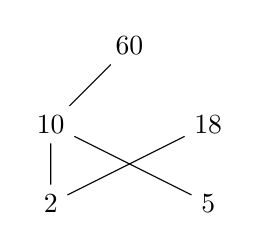
\begin{tikzpicture}
    \node (2) at (0,0) {$2$};
    \node (5) at (2,0) {$5$};
    \node (10) at (0,1) {$10$};
    \node (18) at (2,1) {$18$};
    \node (60) at (1,2) {$60$};

    \draw (2) -- (10) -- (60) ;
    \draw (2) -- (18);
    \draw (5) -- (10);
\end{tikzpicture}

\subsection*{b) }

R = 
$\begin{pmatrix} 
1&0&1&1&1\\
0&1&1&0&1\\
0&0&1&0&1\\ 
0&0&0&1&0\\
0&0&0&0&1\\

\end{pmatrix}$


\subsection*{c) }
For the symmetric closure of R, $R_s$, the matrix should be symmetric, for the diagonal. Hence,

$R_s = 
\begin{pmatrix} 
1&0&1&1&1\\
0&1&1&0&1\\
1&1&1&0&1\\ 
1&0&0&1&0\\
1&1&1&0&1\\
\end{pmatrix}$\\\\

If we utilize XOR from the logic,\\\\

$R \bigoplus R_s = 
\begin{pmatrix} 
0&0&0&0&0\\
0&0&0&0&0\\
1&1&0&0&0\\ 
1&0&0&0&0\\
1&1&1&0&0\\
\end{pmatrix}$\\\\

Hence, our pairs are (10,2), (10,5), (18,2), (60,2), (60,5), and (60,10).

\subsection*{d) }

If we remove and add one node, we cannot get a total ordering since we cannot form a pure chain, they cross all the time. However, if we remove two values, for example, 5 and 18, and add 20, we get a total ordering.\\\\

Chain:
$2|10, 10|60$ or $2|20, 20|60$ 

\end{document}
